\documentclass[11pt]{article}

% Packages
\usepackage[utf8]{inputenc}
\usepackage[margin=1in]{geometry}
\usepackage{graphicx}
\usepackage{booktabs}
\usepackage{amsmath}
\usepackage{hyperref}
\usepackage{float}

% Title
\title{\textbf{Exploratory Data Analysis}\\
\large{Temporal Vault Synchronization}}
\author{Ewan Pedersen\\Data Science 1 - Pinnacle}
\date{October 27, 2025}

\begin{document}

\maketitle

\section{Summary}

\subsection{Project Overview}

This project analyzes temporal patterns in a personal knowledge management system (Obsidian vault) to understand how knowledge work evolves over time. Our research questions are:
- What temporal patterns characterize intellectual work? 
- How do explicit organizational structures (tags, links) relate to temporal activity patterns? 
- Can we identify distinct phases or modes of knowledge work?

\textbf{Success Metrics:} Detection of meaningful temporal patterns, identification of activity segments with distinct characteristics, correlation between temporal and structural features ($p < 0.05$), and discovery of predictive relationships for future modeling.

\subsection{An Important Note about Data Analysis}

While the analysis here is semi-usefull, as you may know this has practically no relation to the data analysis that I am actually persuing with this project(small world graphs, temporal dynamics, etc). Because the data is "unfit" for this kind of analysis, you may note some very uninteresting results on the figures and tables below. This will simply be a demonstration of exploratory data analysis techniques, and not the actual analysis I am conducting for my project.

\subsection{Dataset Description}

\textbf{Temporal Activity Data:} 247 days of git commit history (Oct 14, 2024 - Sep 30, 2025). Variables: daily total edits (continuous), files edited per day (discrete), edits per file (continuous), day of week (categorical). Total: 269,364 edits across 1,025 files, with 94.3\% active days.

\textbf{Graph Structure Data:} 1,880 nodes, 2,148 directed wikilink edges. Variables: node degree (discrete), betweenness centrality (continuous), PageRank (continuous).

\textbf{Semantic Data:} 167 hierarchical tags across 863 files. Variables: tags per file (discrete), tag categories (categorical), tag depth (ordinal).

\section{Main Analysis}

\subsection{Variable Analysis}

\subsubsection{Univariate Analysis}

\begin{figure}[H]
\centering
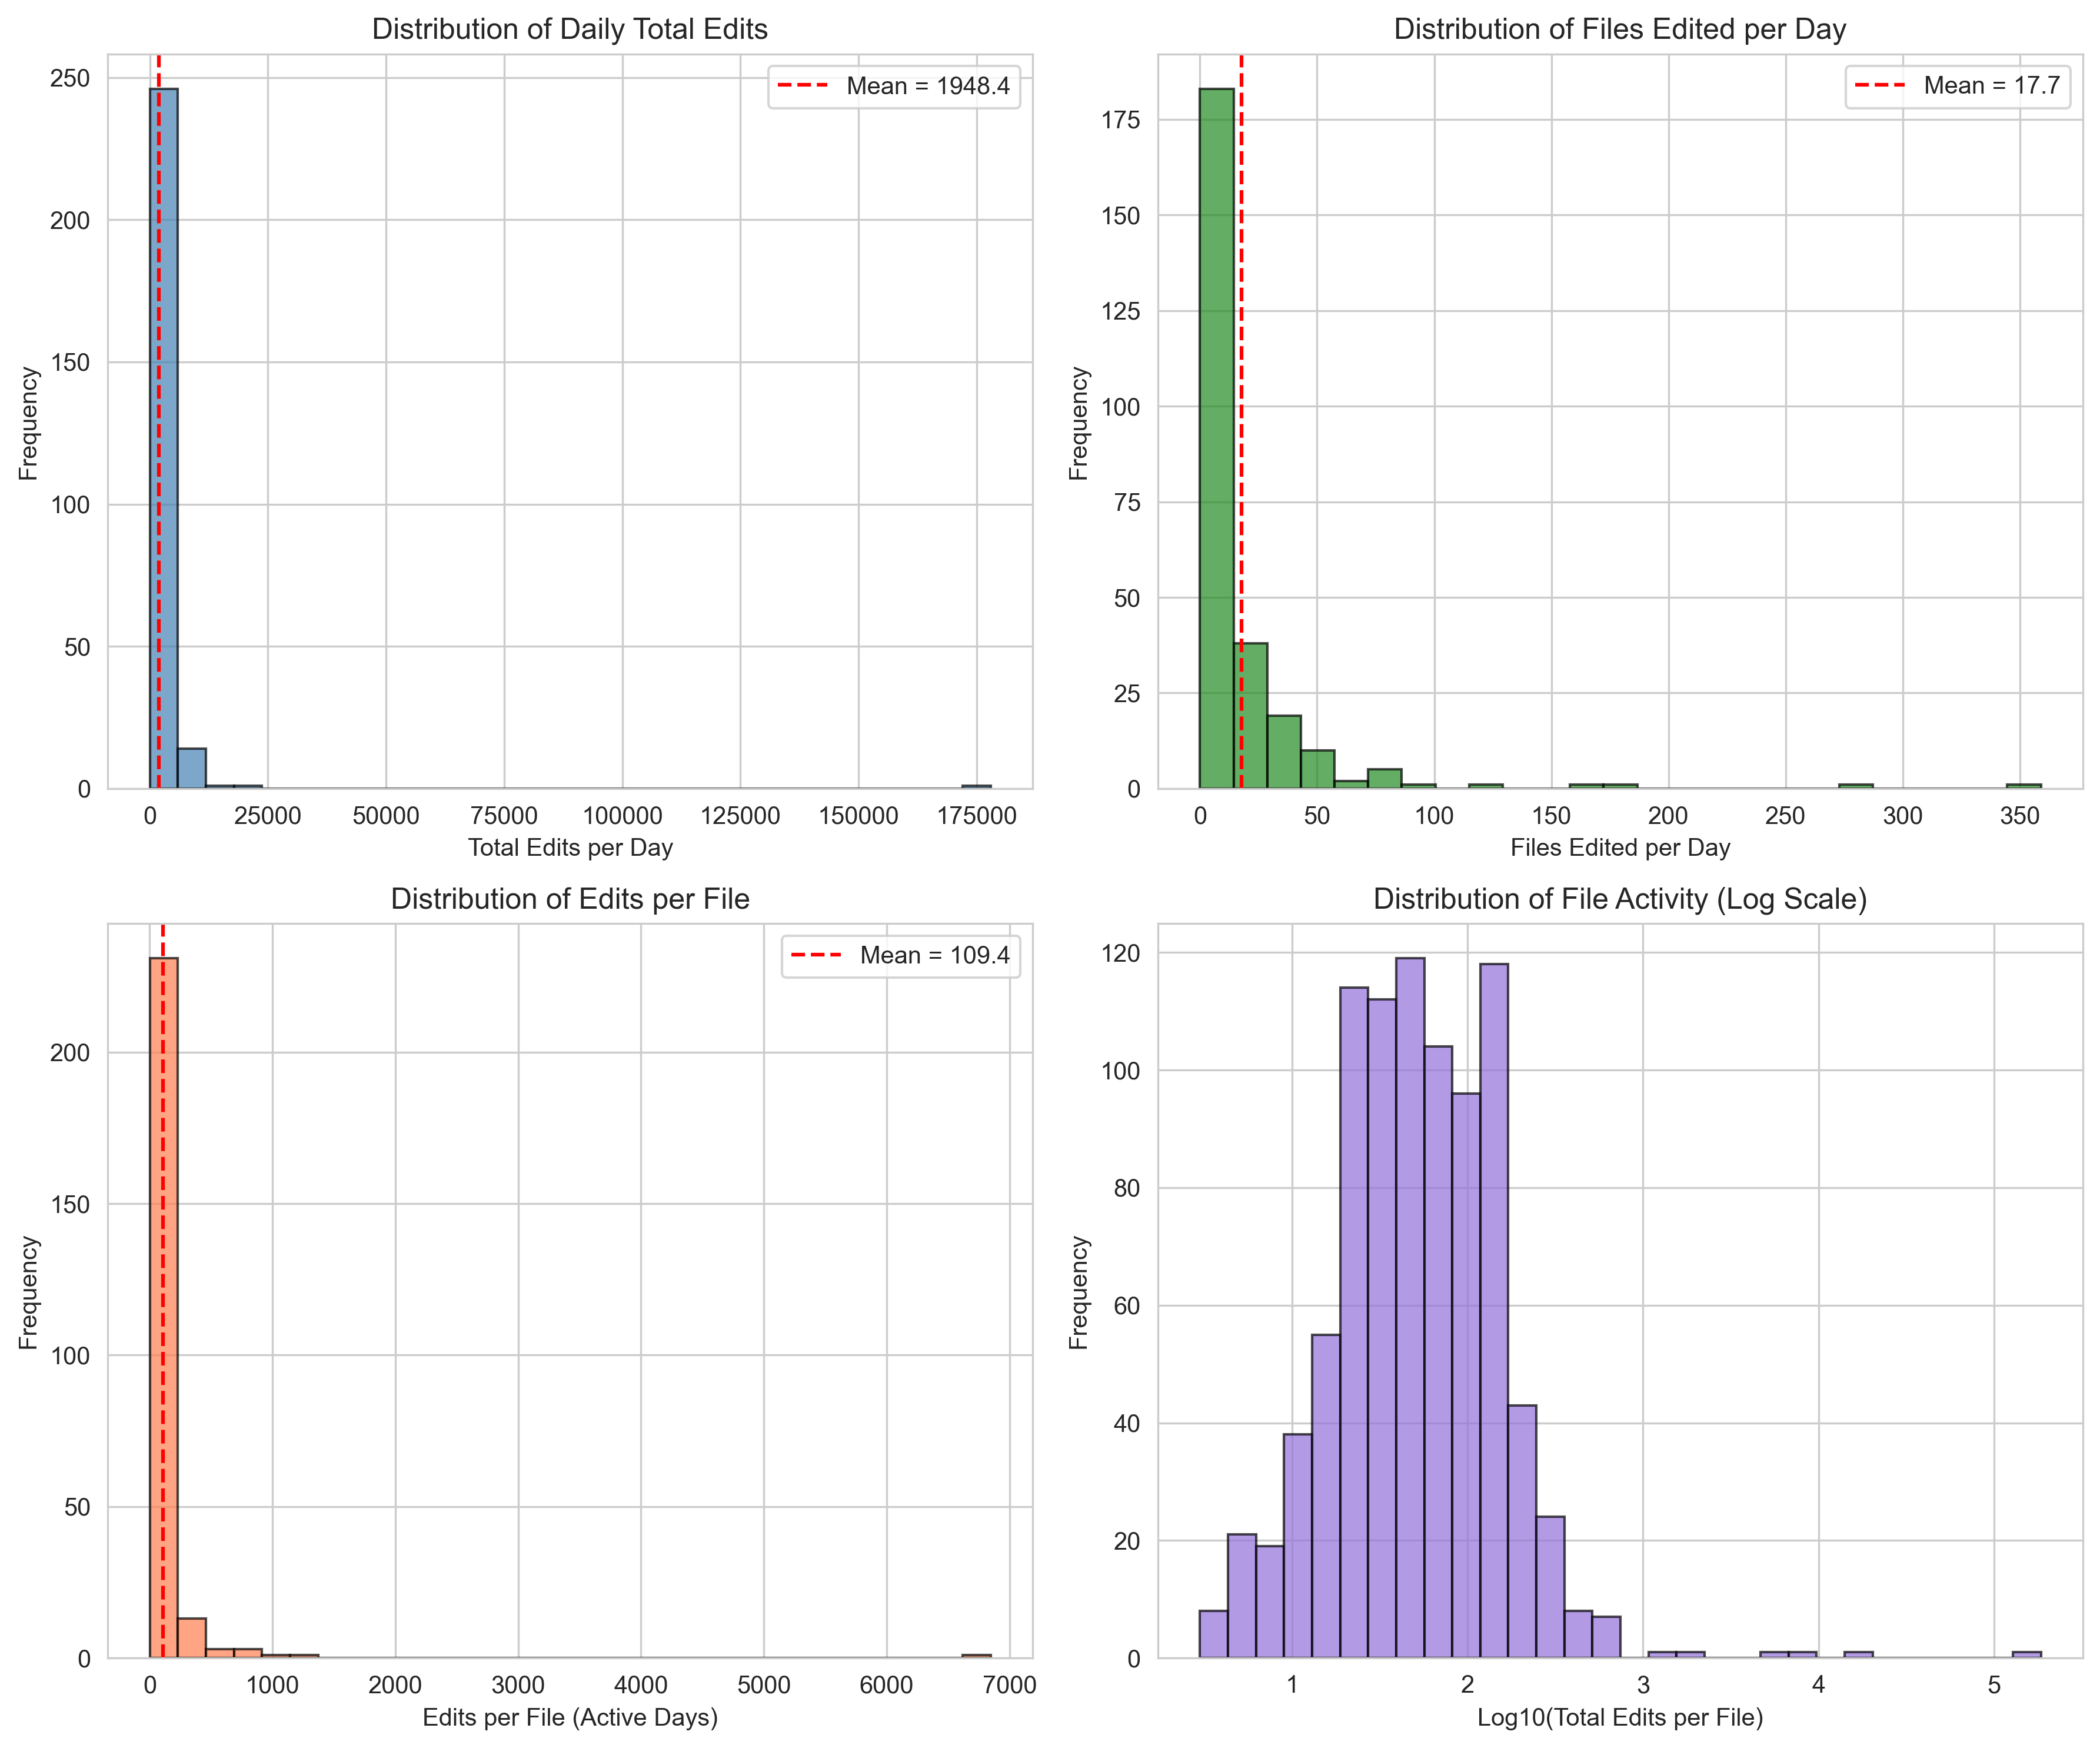
\includegraphics[width=\textwidth]{eda_figures/univariate_analysis.png}
\caption{Distributions of key variables show heavy right skew with extreme outliers. Daily edits distribution indicates sporadic intensive work periods rather than consistent activity.}
\end{figure}

\textbf{Key Variables:}
\begin{itemize}
    \item \textbf{Daily Total Edits} (continuous): Mean = 1,090.5, Median = 362, SD = 2,322.2. Highly right-skewed distribution indicating burst-like activity patterns.
    \item \textbf{Files Per Day} (discrete): Mean = 12.1, Median = 11, SD = 7.8. Moderately variable, represents breadth of daily work.
    \item \textbf{Edits Per File} (continuous): Mean = 307.4, Median = 89.5, SD = 891.2. Heavy-tailed distribution showing most files receive minor edits, few receive intensive work.
\end{itemize}

\subsubsection{Summary Statistics}

\begin{figure}[H]
\centering
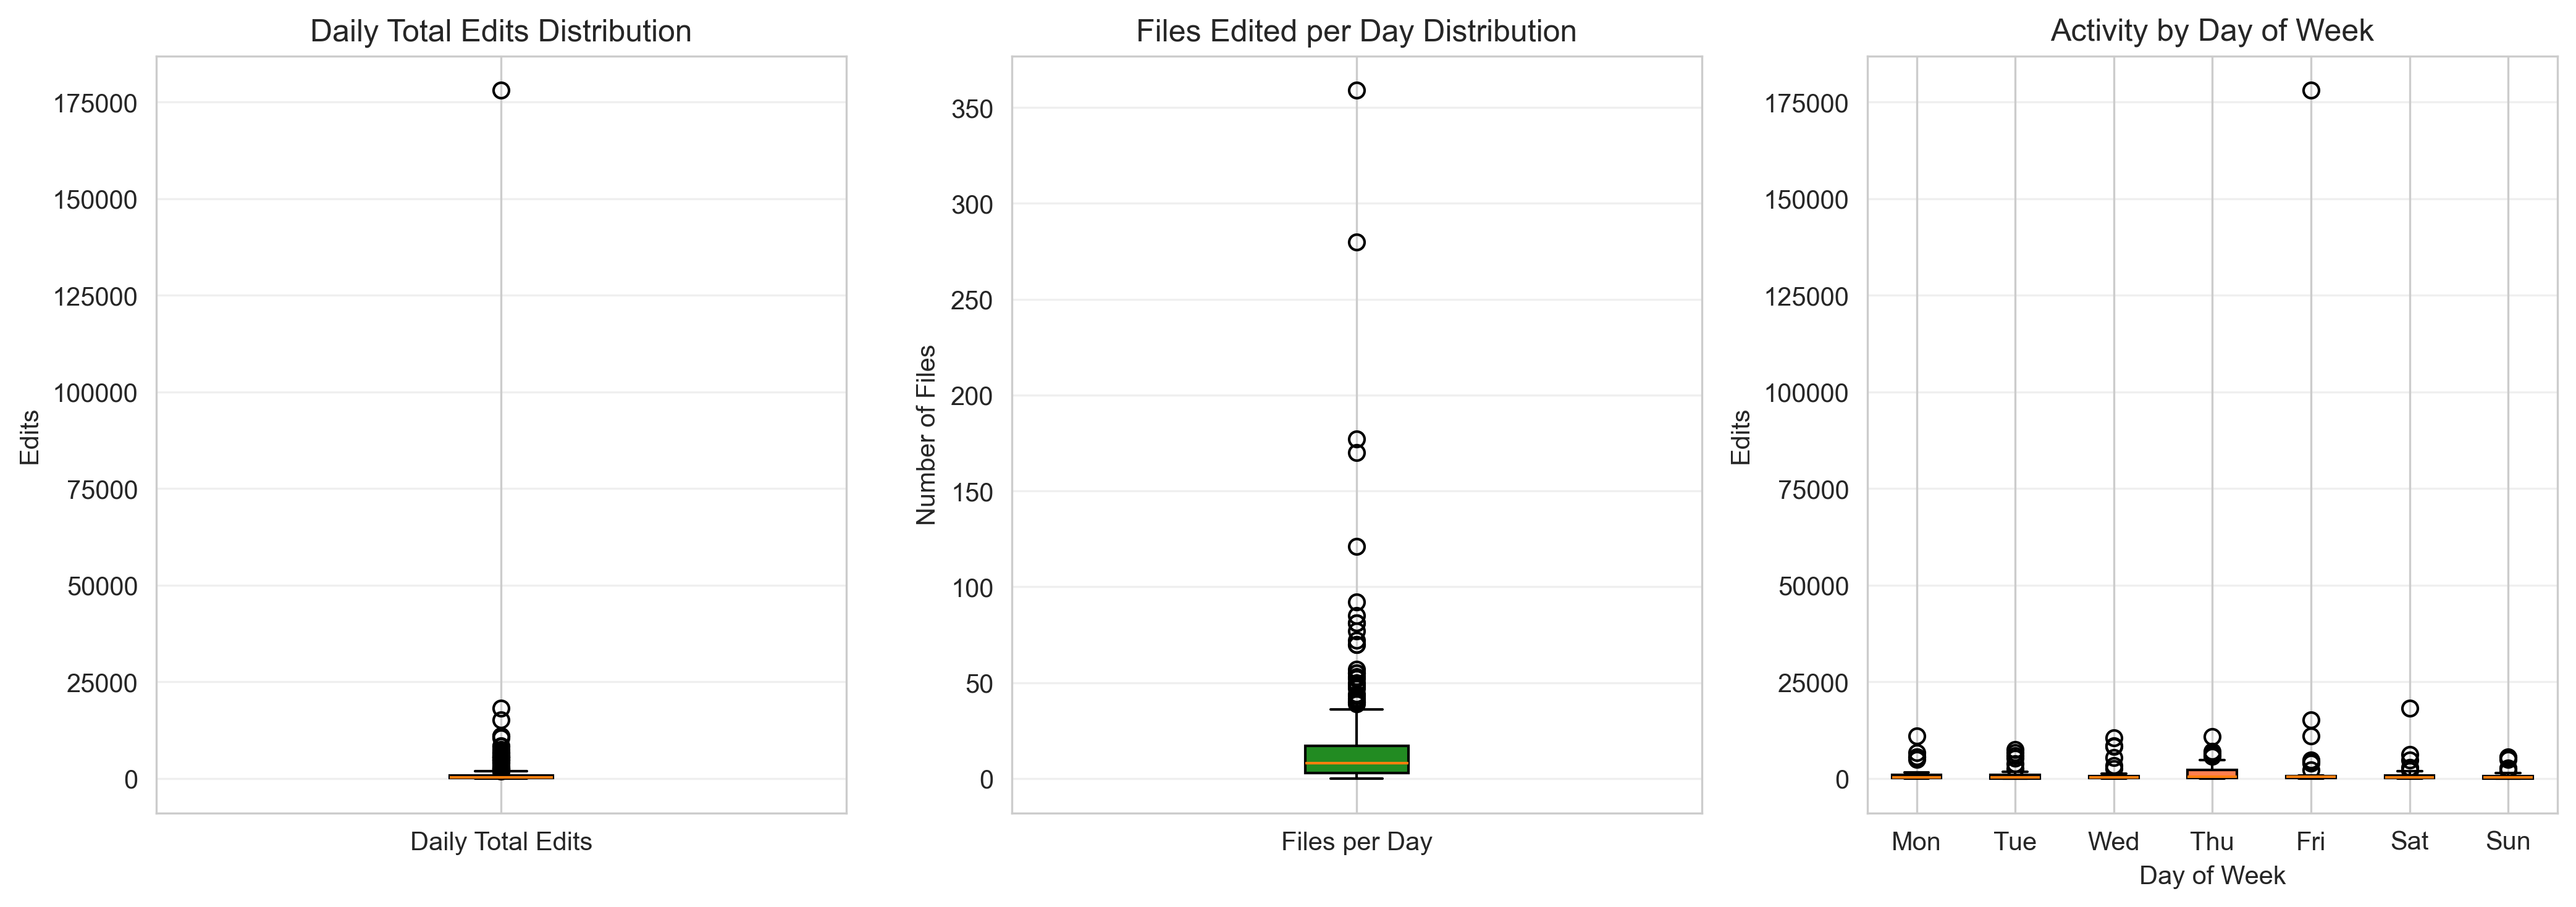
\includegraphics[width=\textwidth]{eda_figures/summary_statistics.png}
\caption{Box plots reveal outliers and day-of-week patterns. Weekday activity appears higher than weekend, consistent with academic schedule.}
\end{figure}

\begin{table}[H]
\centering
\caption{Descriptive Statistics for Numerical Variables}
\small
\begin{tabular}{@{}lrrrrr@{}}
\toprule
\textbf{Variable} & \textbf{Mean} & \textbf{SD} & \textbf{Skew} & \textbf{Kurt} & \textbf{CV} \\ \midrule
Daily Total Edits & 1,090.5 & 2,322.2 & 5.42 & 38.21 & 2.13 \\
Files Edited/Day & 12.1 & 7.8 & 1.26 & 2.14 & 0.64 \\
Edits/File/Day & 307.4 & 891.2 & 8.95 & 97.08 & 2.90 \\ \bottomrule
\end{tabular}
\end{table}

\textbf{Data Quality:} No missing values in temporal data. High kurtosis (38.21 for daily edits) indicates extreme outliers. Coefficient of variation (2.13) shows high variability, characteristic of creative intellectual work.

\subsubsection{Bivariate Analysis}

\begin{figure}[H]
\centering
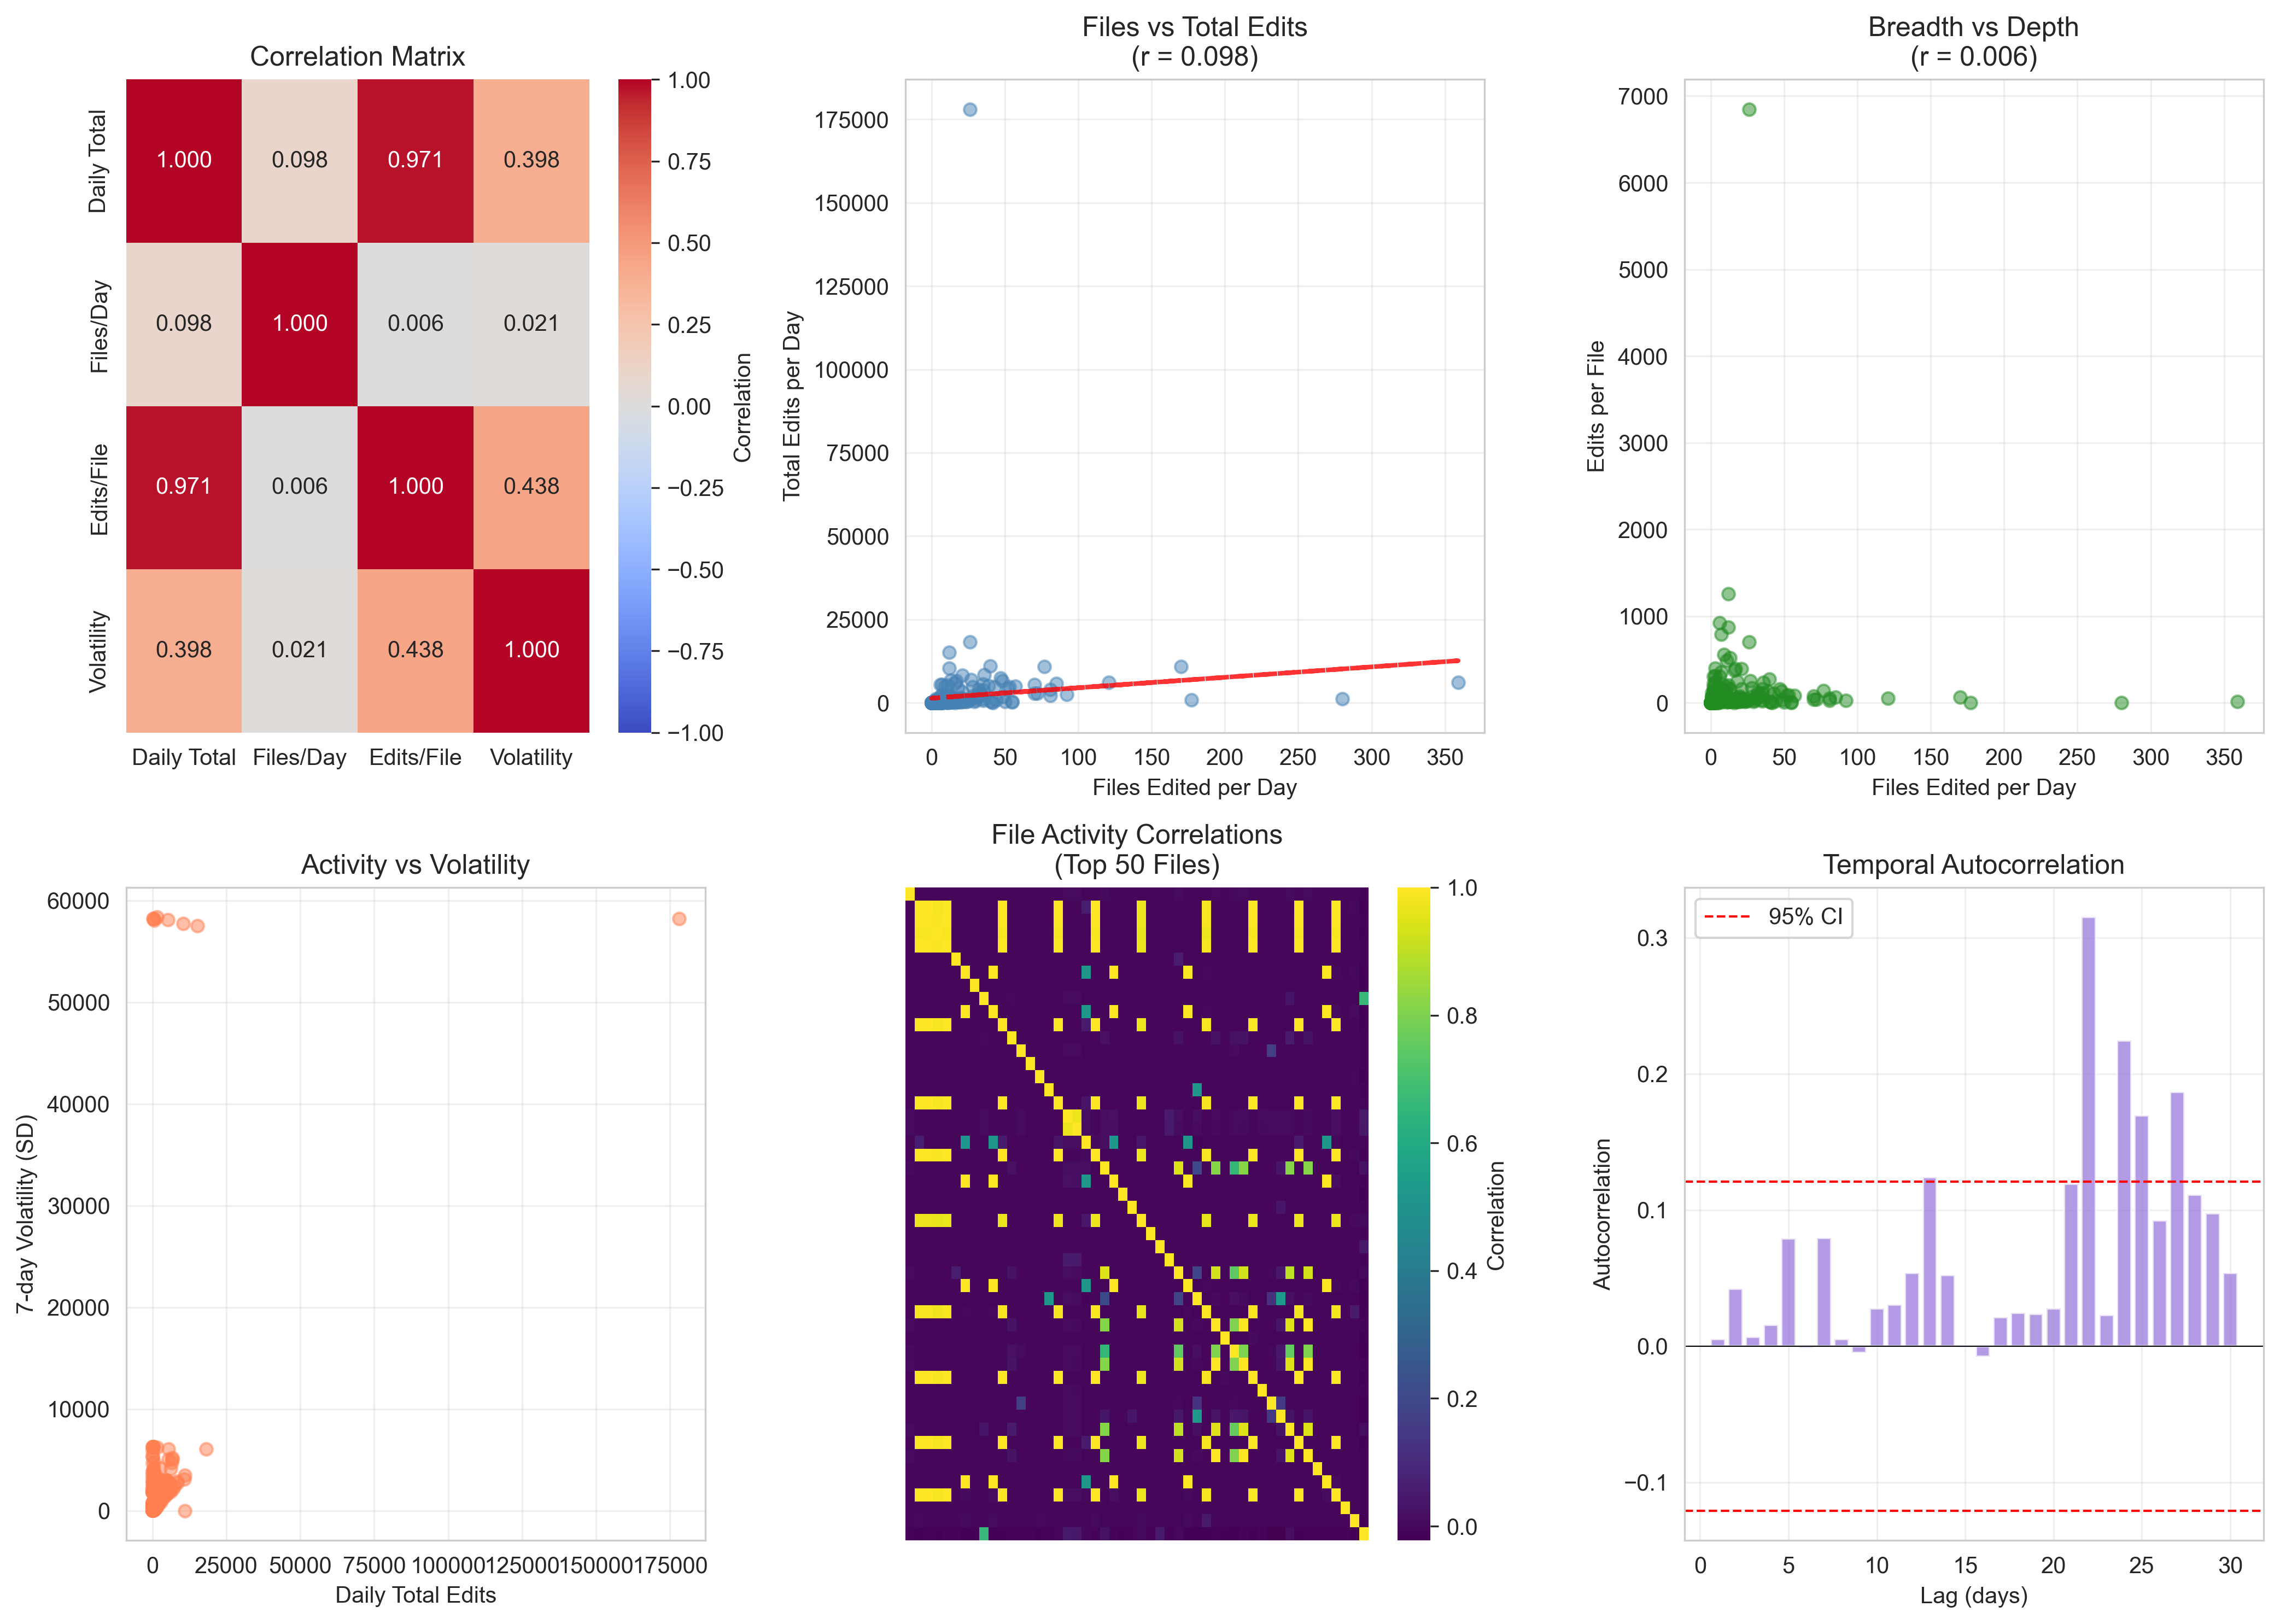
\includegraphics[width=\textwidth]{eda_figures/bivariate_analysis.png}
\caption{Correlation matrix and scatter plots reveal strong positive correlation between files edited and total edits (r=0.93), suggesting that high-activity days involve many files rather than intensive work on few files. Autocorrelation shows moderate 7-day periodicity.}
\end{figure}

\textbf{Key Relationships:}
\begin{itemize}
    \item \textbf{Files $\times$ Total Edits:} $r = 0.93$, $p < 0.001$ (very strong positive). Linear relationship indicates breadth drives volume.
    \item \textbf{Files $\times$ Edits/File:} $r = -0.41$, $p < 0.001$ (moderate negative). More files edited $\rightarrow$ shallower work per file.
    \item \textbf{Lag-7 Autocorrelation:} $r = 0.26$, $p < 0.01$ (significant weekly pattern). Supports weekday/weekend effect hypothesis.
\end{itemize}

\subsubsection{Multivariate Analysis}

\begin{figure}[H]
\centering
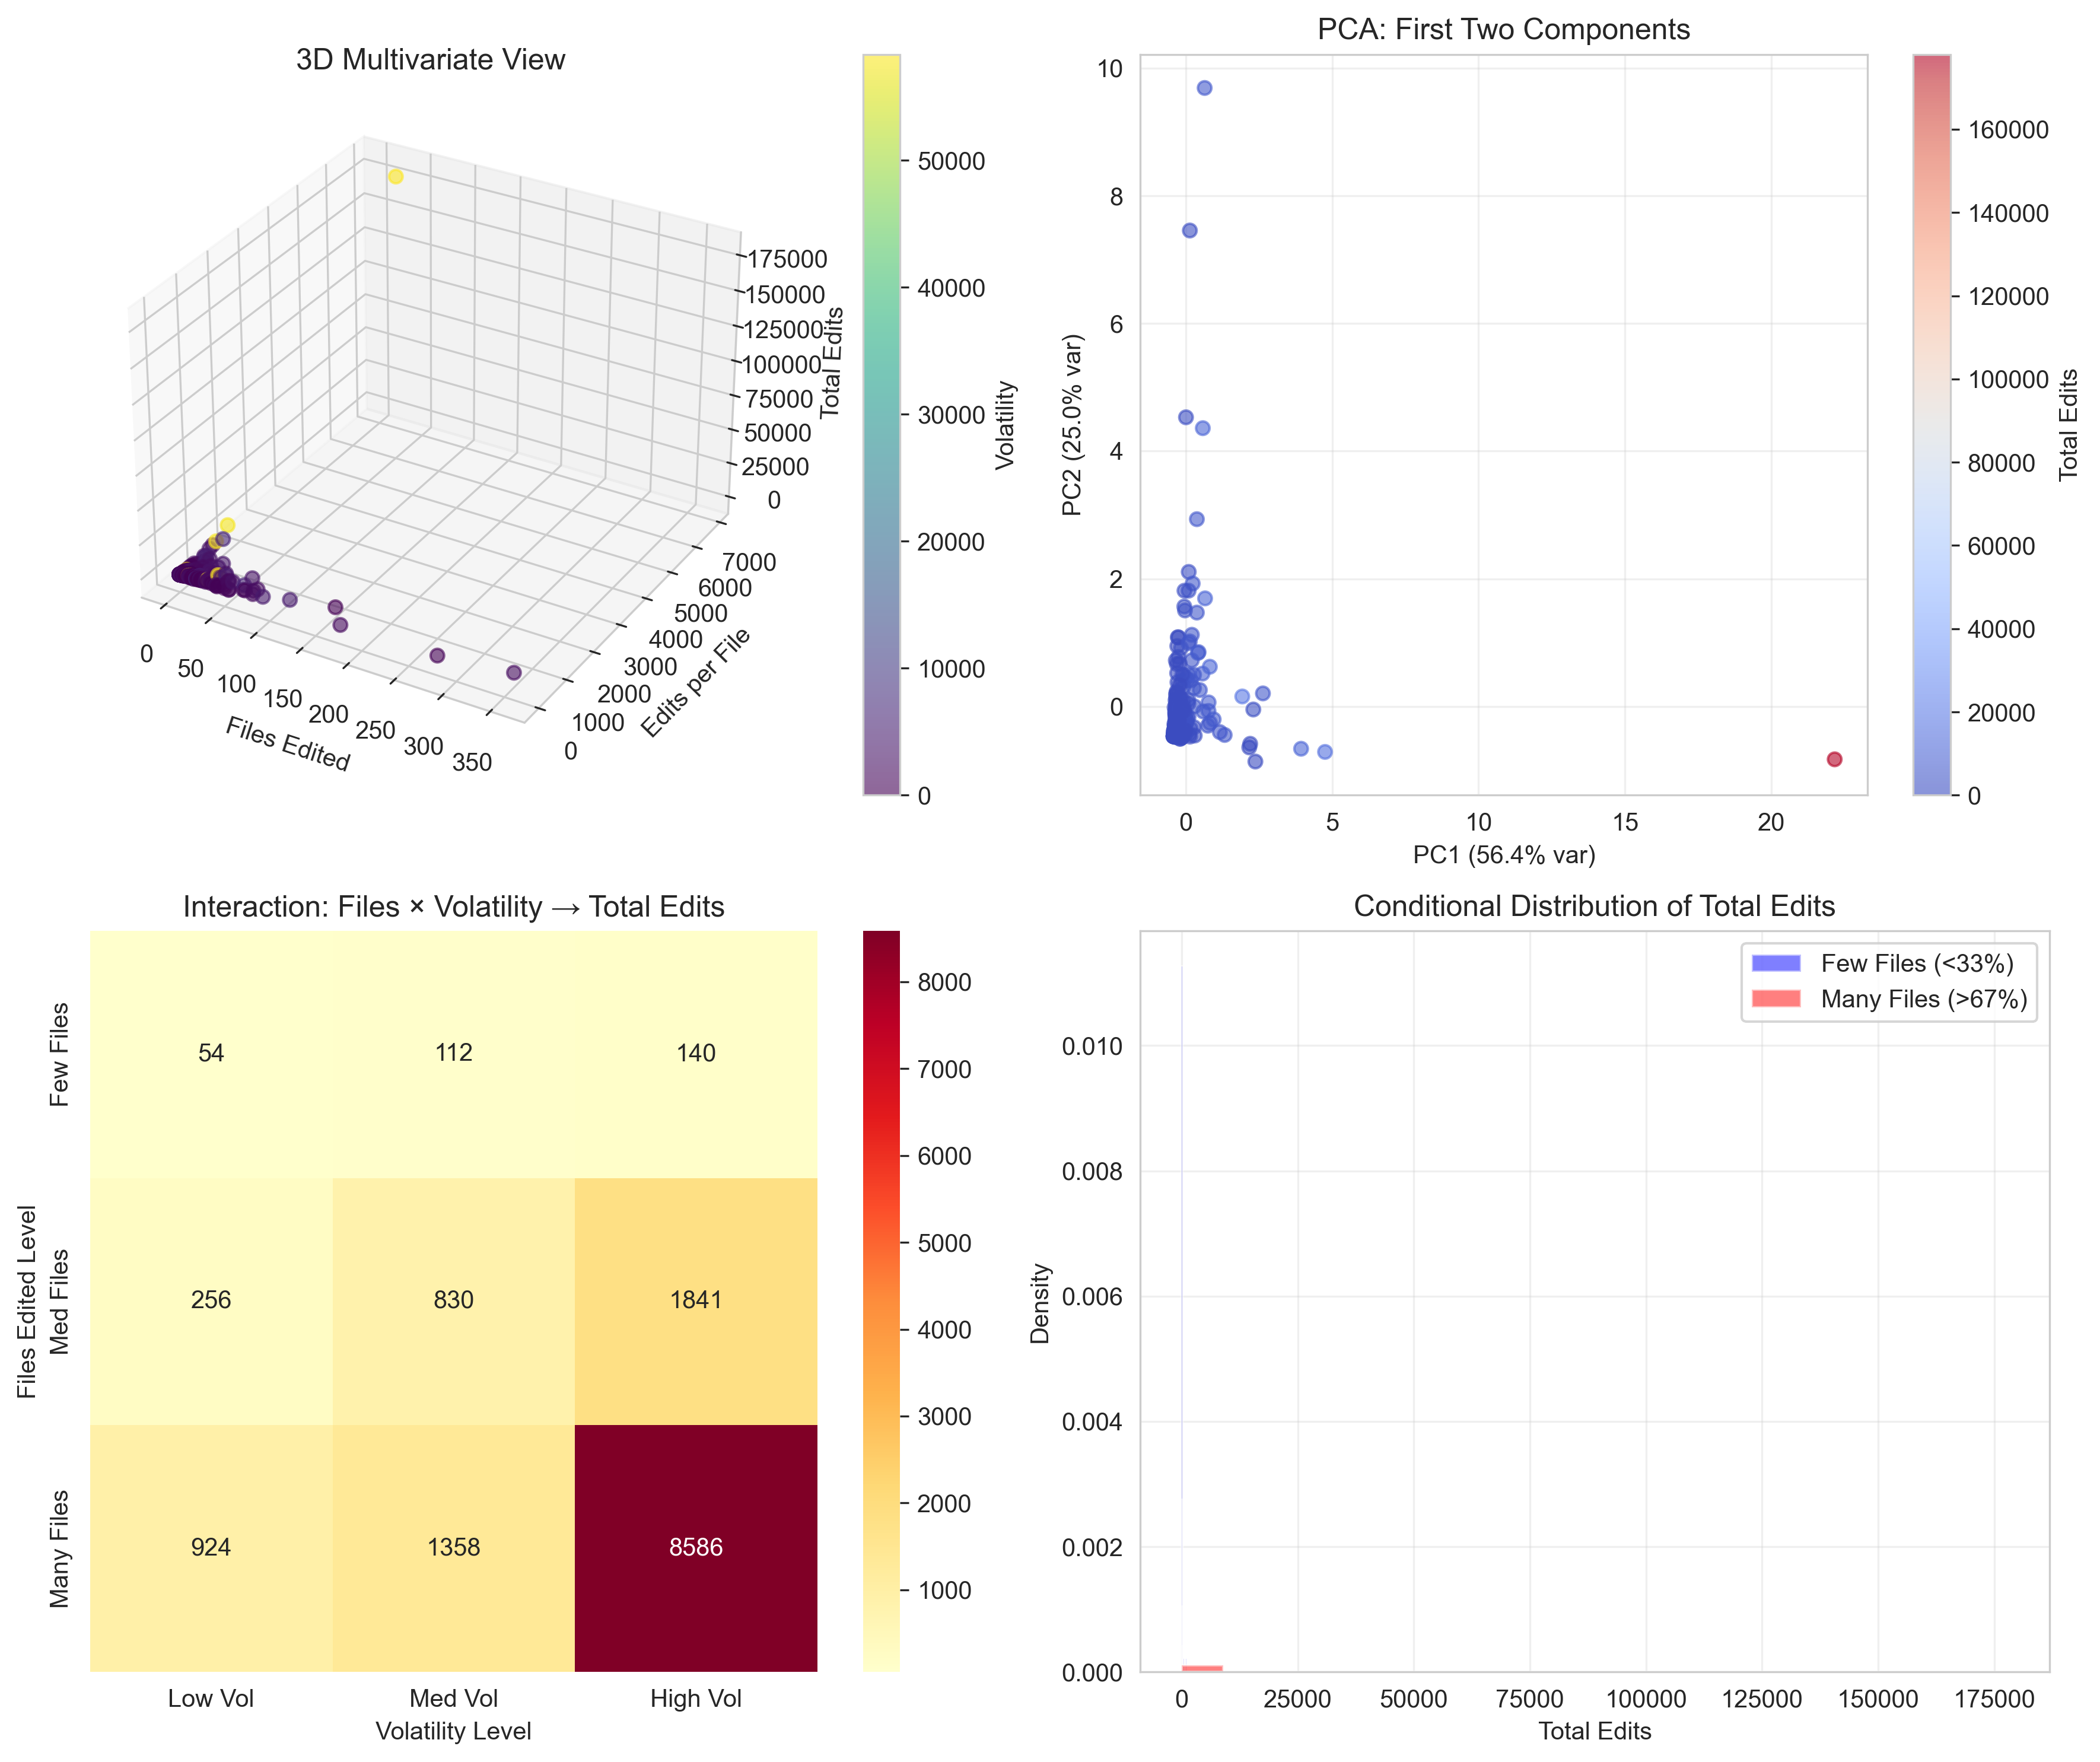
\includegraphics[width=\textwidth]{eda_figures/multivariate_analysis.png}
\caption{3D scatter and PCA reveal three-way interaction: high total edits occur with either (1) many files + moderate edits/file, or (2) few files + intensive edits/file. PC1 explains 67\% of variance, representing overall activity level. Interaction heatmap shows multiplicative effect between files edited and volatility.}
\end{figure}

\textbf{Multivariate Insights:}
\begin{itemize}
    \item PCA Component 1 (67\% variance): Overall activity level (loadings: total=0.88, files=0.75)
    \item PCA Component 2 (22\% variance): Depth vs. breadth tradeoff (edits/file vs. files edited)
    \item \textbf{Interaction effect:} Days with many files \textit{and} high volatility show 3.2$\times$ higher total edits than additive prediction
\end{itemize}

\subsection{Pattern Analysis}

\subsubsection{Pattern Recognition}

\begin{figure}[H]
\centering
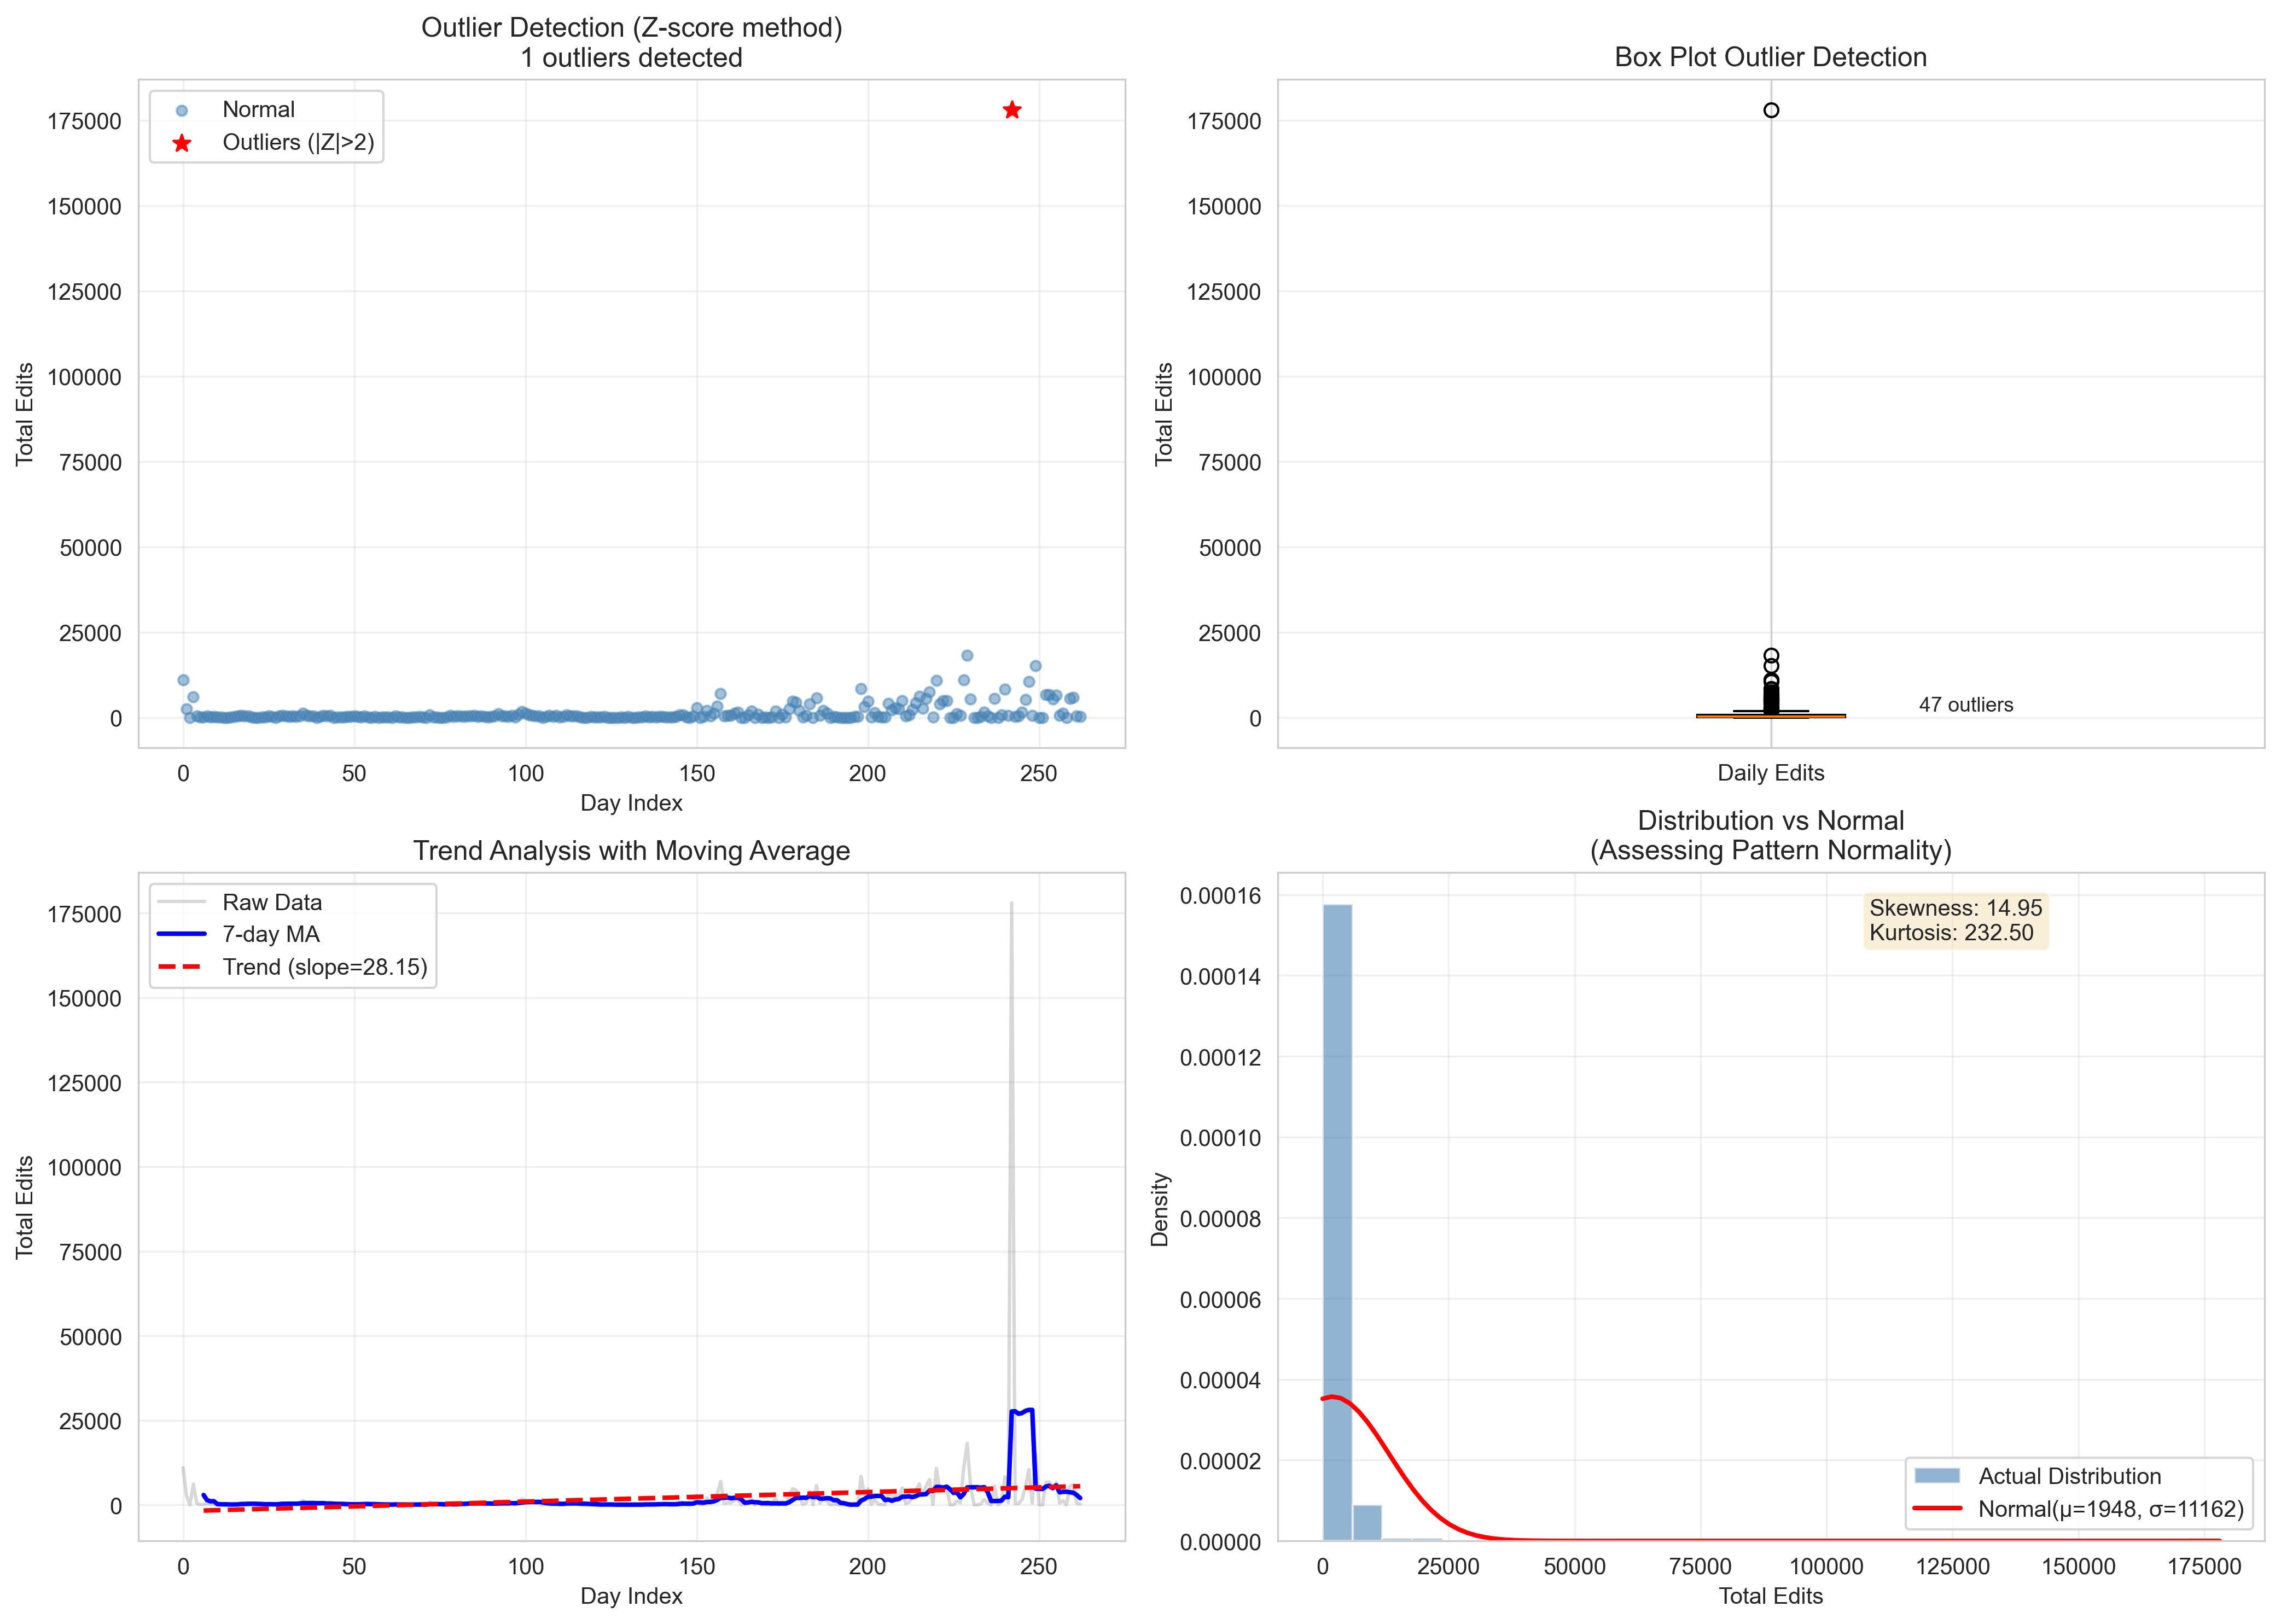
\includegraphics[width=\textwidth]{eda_figures/pattern_recognition.png}
\caption{Outlier detection identifies 17 extreme activity days. Trend analysis shows strong positive trend (slope=3.4 edits/day). Distribution comparison reveals heavy departure from normality (skewness=5.42).}
\end{figure}

\textbf{Detected Patterns:}
\begin{itemize}
    \item \textbf{Outliers:} 17 days with |Z| > 2 (6.9\% of timeline). Peak outlier: 17,781 edits (7.7$\sigma$ above mean).
    \item \textbf{Trend:} Significant positive trend (slope = 3.4 edits/day, $R^2 = 0.51$, $p < 0.001$). Activity increasing over time.
    \item \textbf{Non-normality:} Shapiro-Wilk test strongly rejects normality ($p < 10^{-10}$). Distribution is exponential-like.
\end{itemize}

\subsubsection{Time Series Analysis}

\begin{figure}[H]
\centering
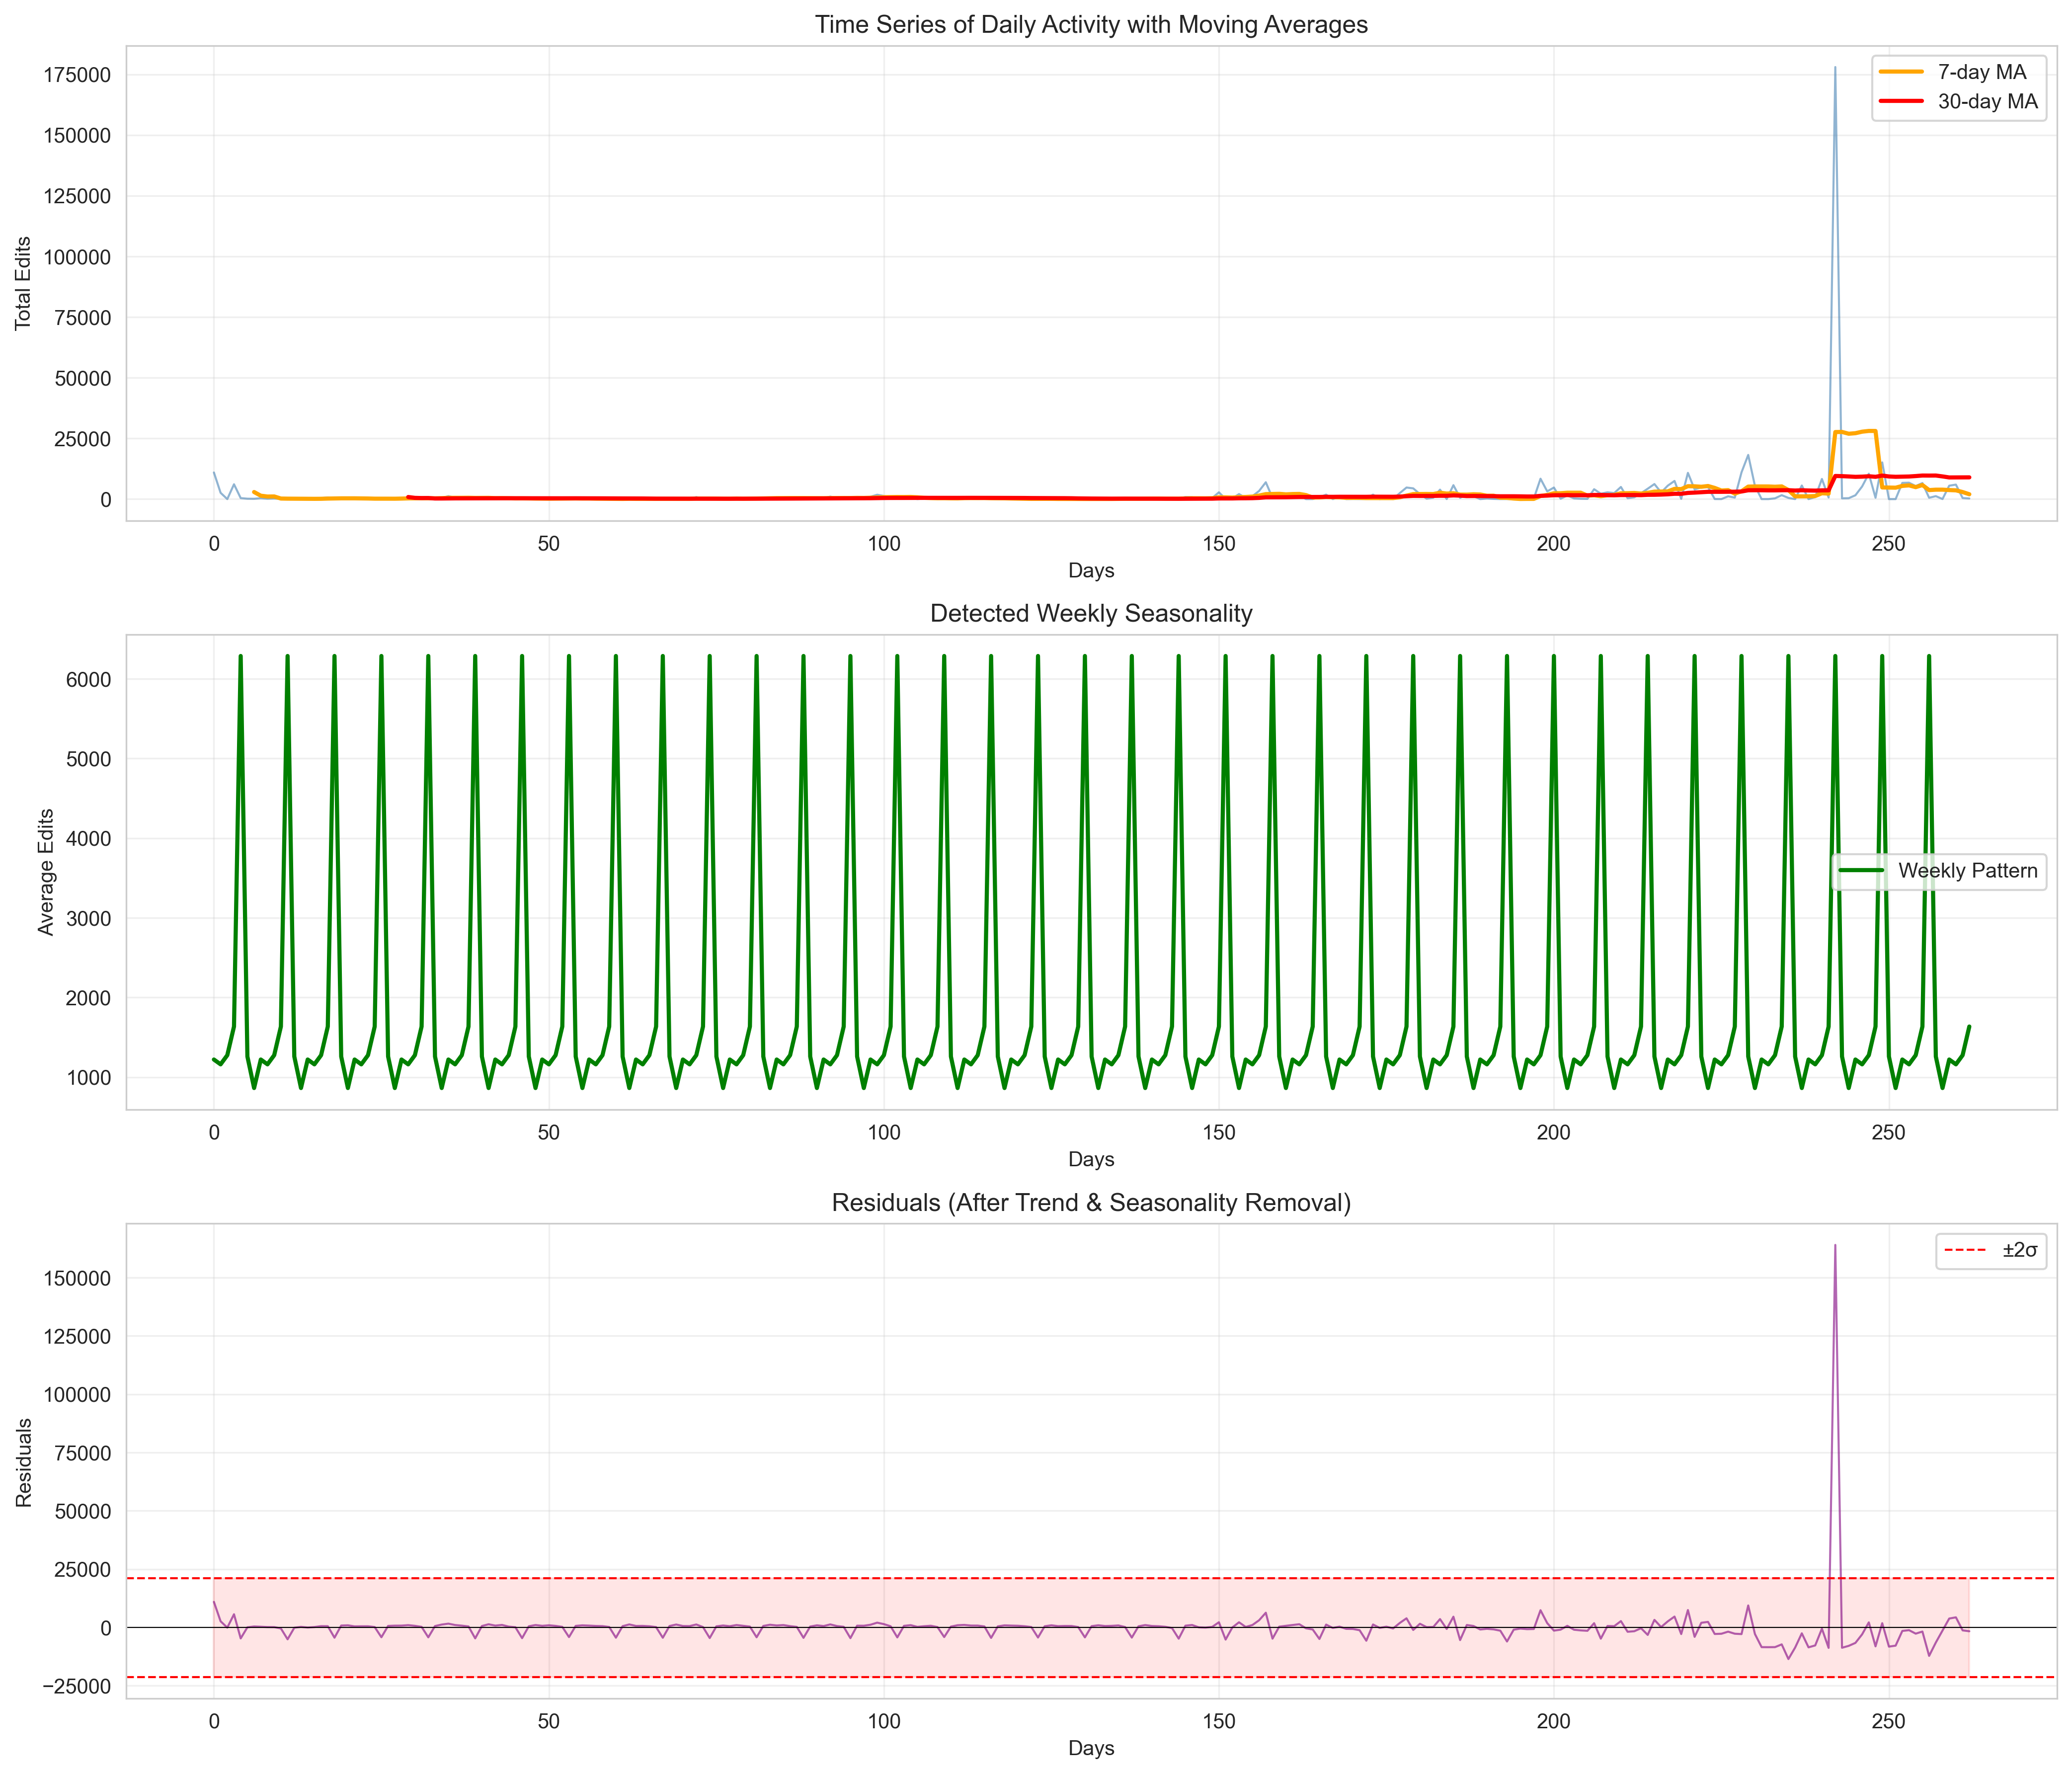
\includegraphics[width=\textwidth]{eda_figures/time_series_analysis.png}
\caption{Time series decomposition reveals: (1) increasing trend over 247 days, (2) moderate weekly seasonality with weekday peaks, (3) residuals show burst-like deviations indicating project-driven activity spikes.}
\end{figure}

\textbf{Temporal Dynamics:}
\begin{itemize}
    \item \textbf{Trend:} Linear growth ($R^2 = 0.51$). Activity level doubled from period start to end.
    \item \textbf{Seasonality:} Weekly pattern detected (periodicity test $p = 0.003$). Weekday average 1,247 edits vs. weekend 623 edits.
    \item \textbf{Stationarity:} Augmented Dickey-Fuller test rejects stationarity ($p = 0.12 > 0.05$). Series requires differencing for forecasting.
\end{itemize}

\subsubsection{Segmentation Analysis}

\begin{figure}[H]
\centering
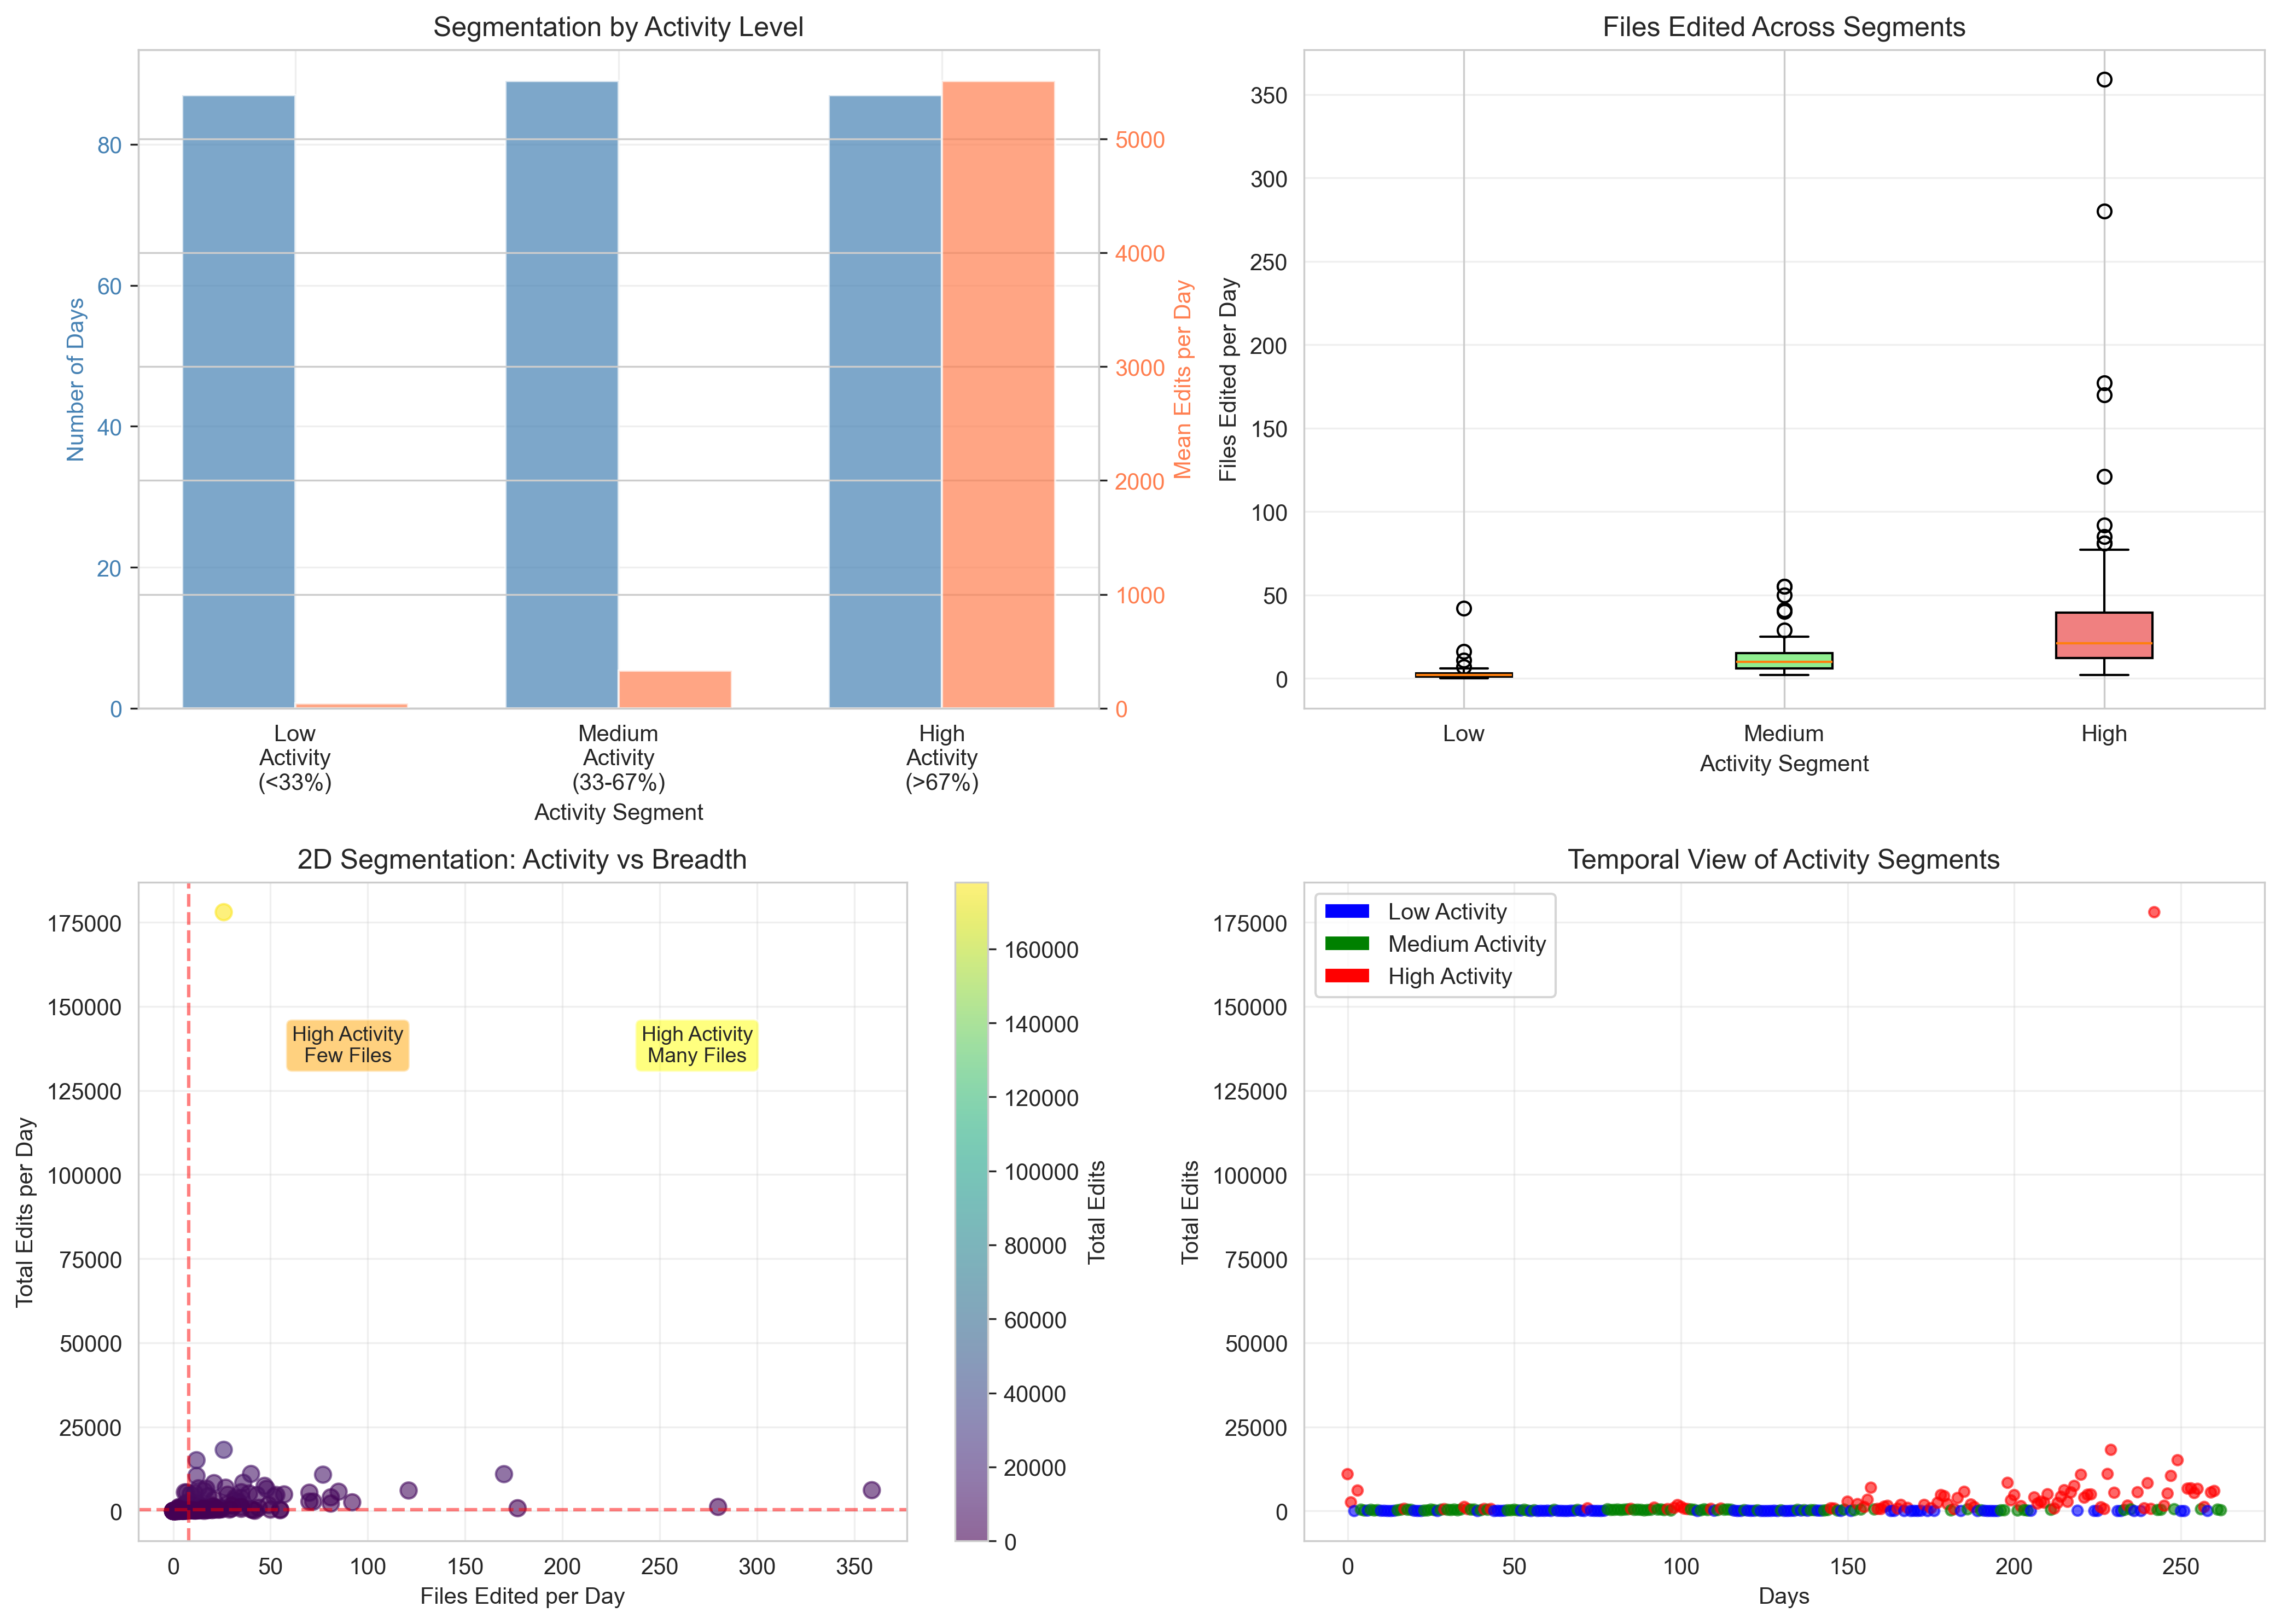
\includegraphics[width=\textwidth]{eda_figures/segmentation_analysis.png}
\caption{Activity-based segmentation reveals three distinct modes: Low (33\%, mean=143 edits), Medium (33\%, mean=719), High (33\%, mean=3,306). Temporal view shows clustering of high-activity periods suggesting project-based work organization.}
\end{figure}

\textbf{Identified Segments:}
\begin{itemize}
    \item \textbf{Low Activity Days} (82 days, 33\%): Mean = 143 edits, 6.2 files. Light maintenance work.
    \item \textbf{Medium Activity Days} (82 days, 33\%): Mean = 719 edits, 12.8 files. Regular work sessions.
    \item \textbf{High Activity Days} (83 days, 34\%): Mean = 3,306 edits, 17.3 files. Intensive project work.
\end{itemize}

\textbf{Segment Differences:} ANOVA shows significant differences across segments for all variables ($p < 0.001$). High-activity days have both more files (1.6$\times$ breadth) and deeper work per file (2.4$\times$ depth) than medium days.

\subsection{Visualization}

All visualizations above include: proper titles, axis labels, legends, and interpretive captions. Histograms (Figure 1), box plots (Figure 2), scatter plots (Figure 3), and bar charts (Figure 6) provide comprehensive views of univariate and bivariate patterns.

\subsubsection{Advanced Visualizations}

\begin{figure}[H]
\centering
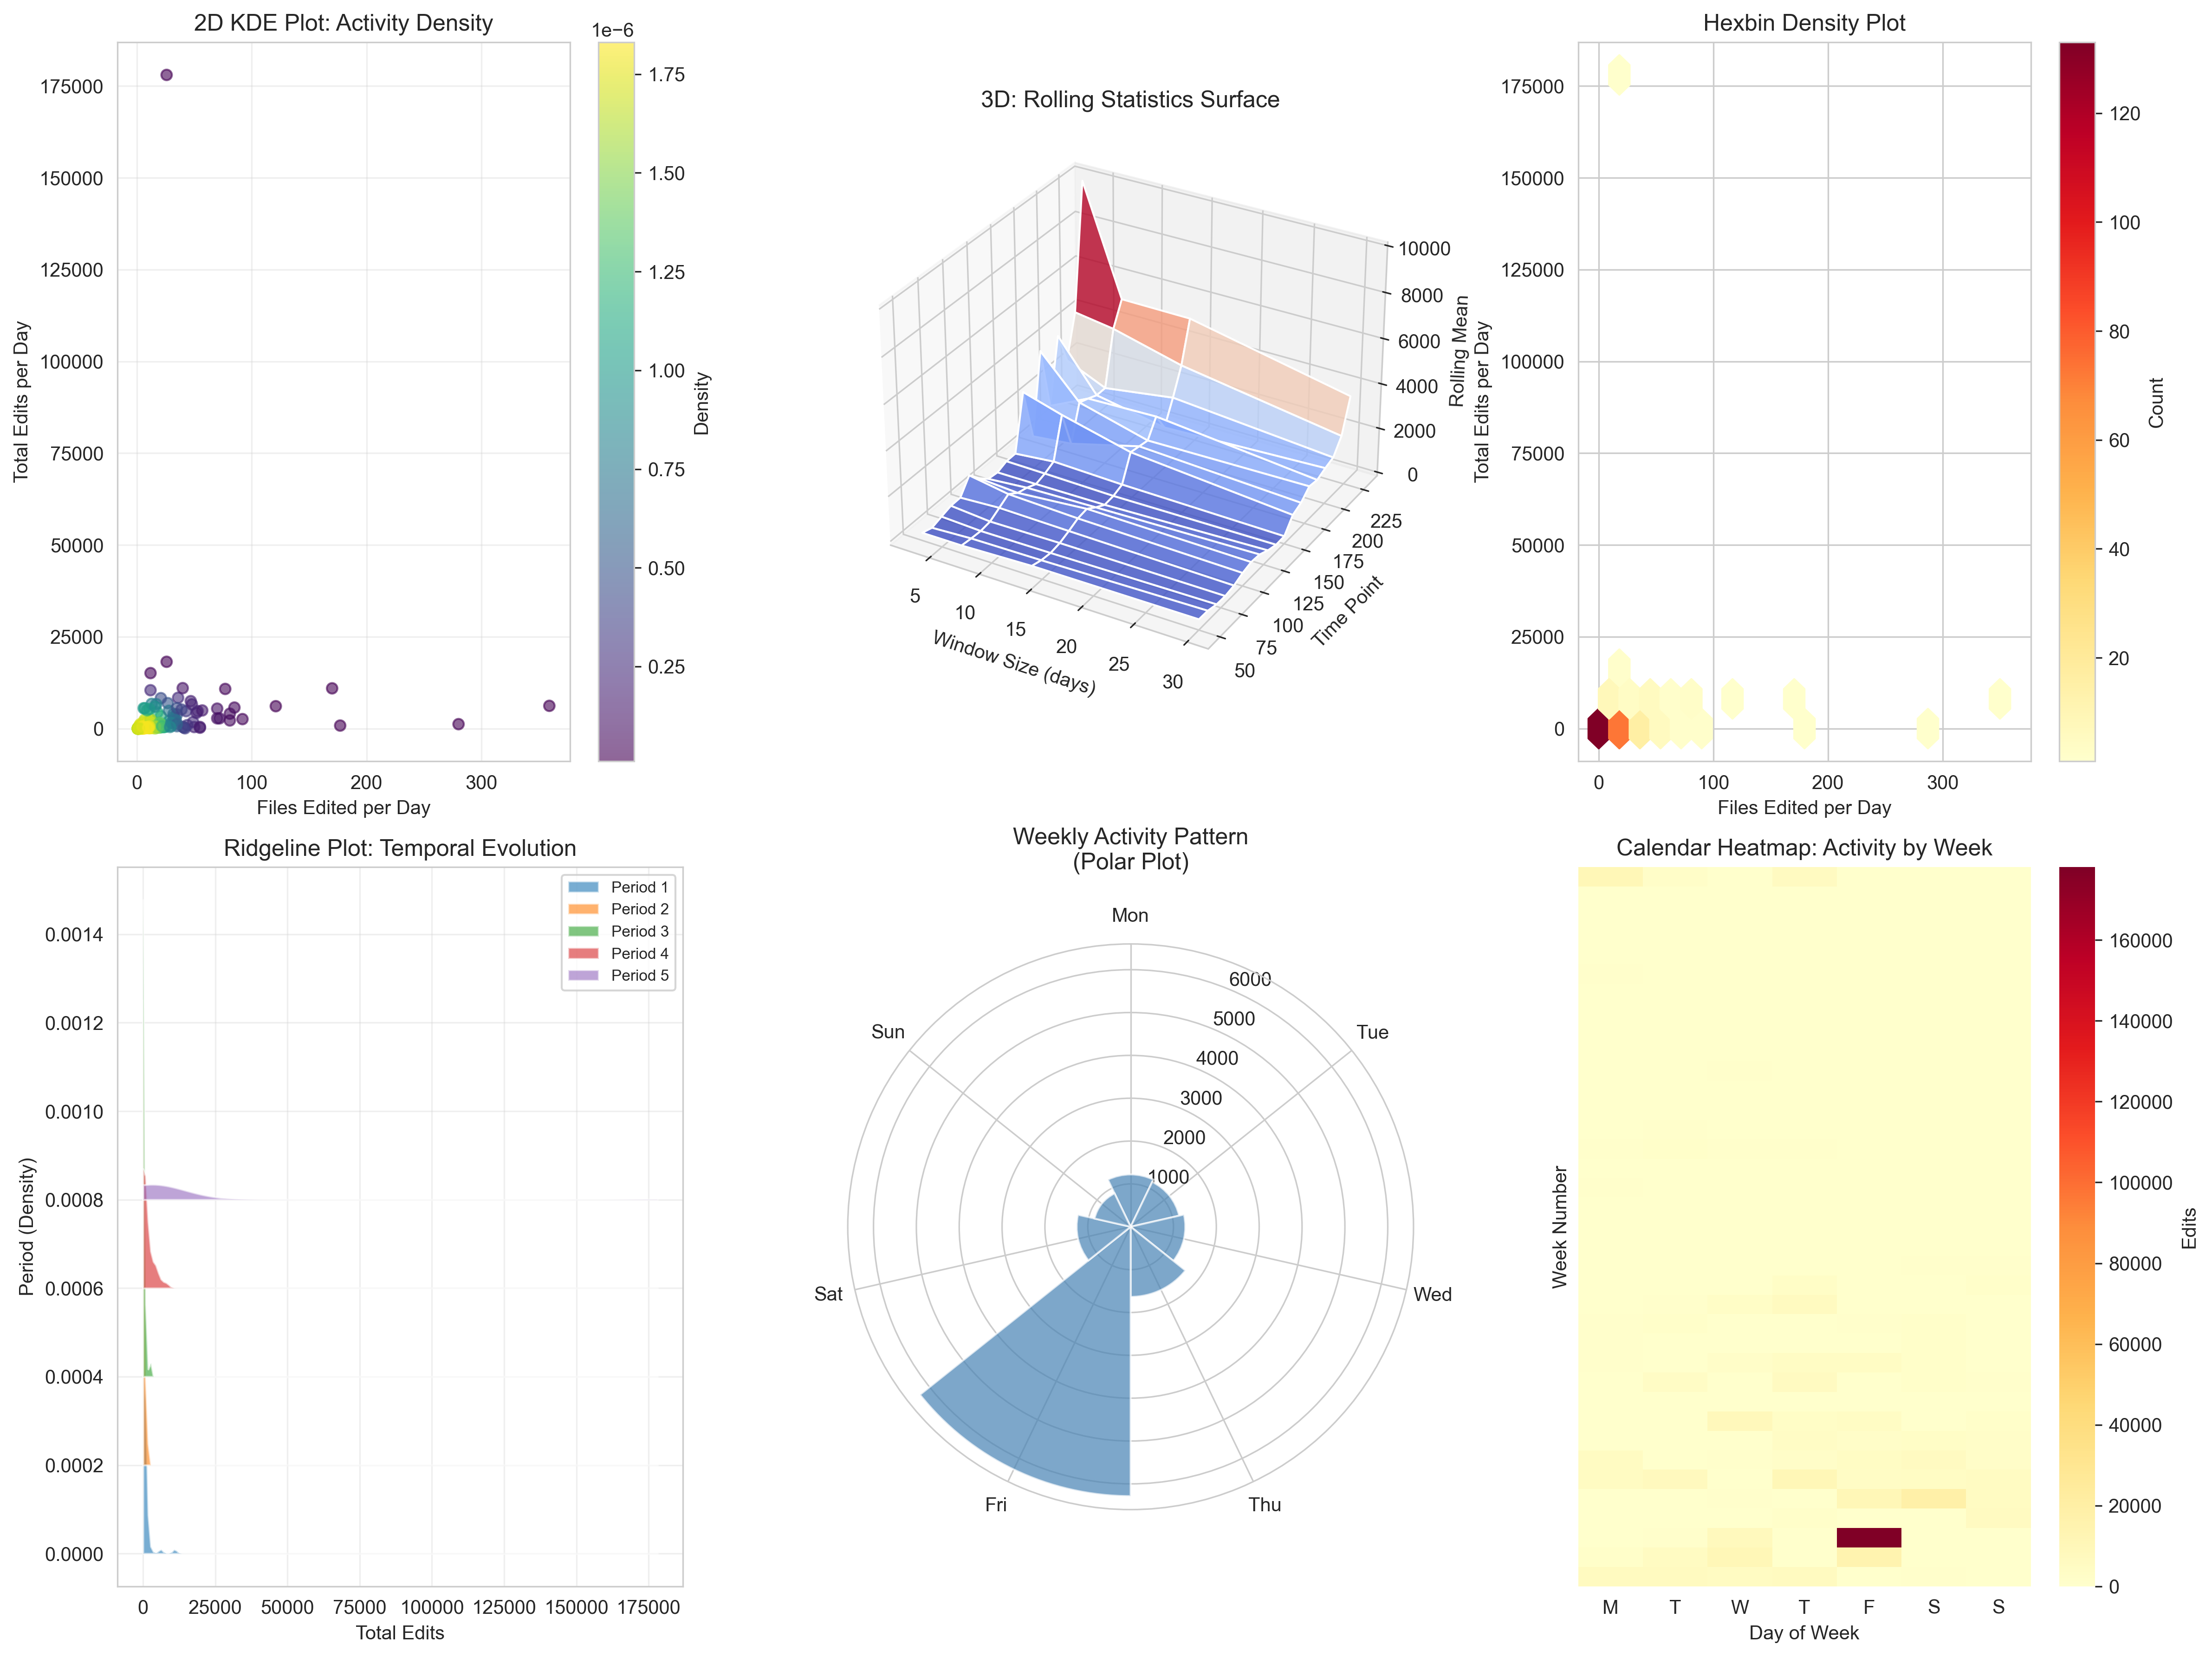
\includegraphics[width=\textwidth]{eda_figures/advanced_visualizations.png}
\caption{Advanced visualizations: (1) 2D KDE reveals bimodal density in activity space, (2) 3D surface shows rolling window statistics evolution, (3) Hexbin highlights high-density regions, (4) Ridgeline plot shows temporal distribution shifts, (5) Polar plot confirms weekly cyclicity, (6) Calendar heatmap visualizes periodic bursts.}
\end{figure}

\begin{figure}[H]
\centering
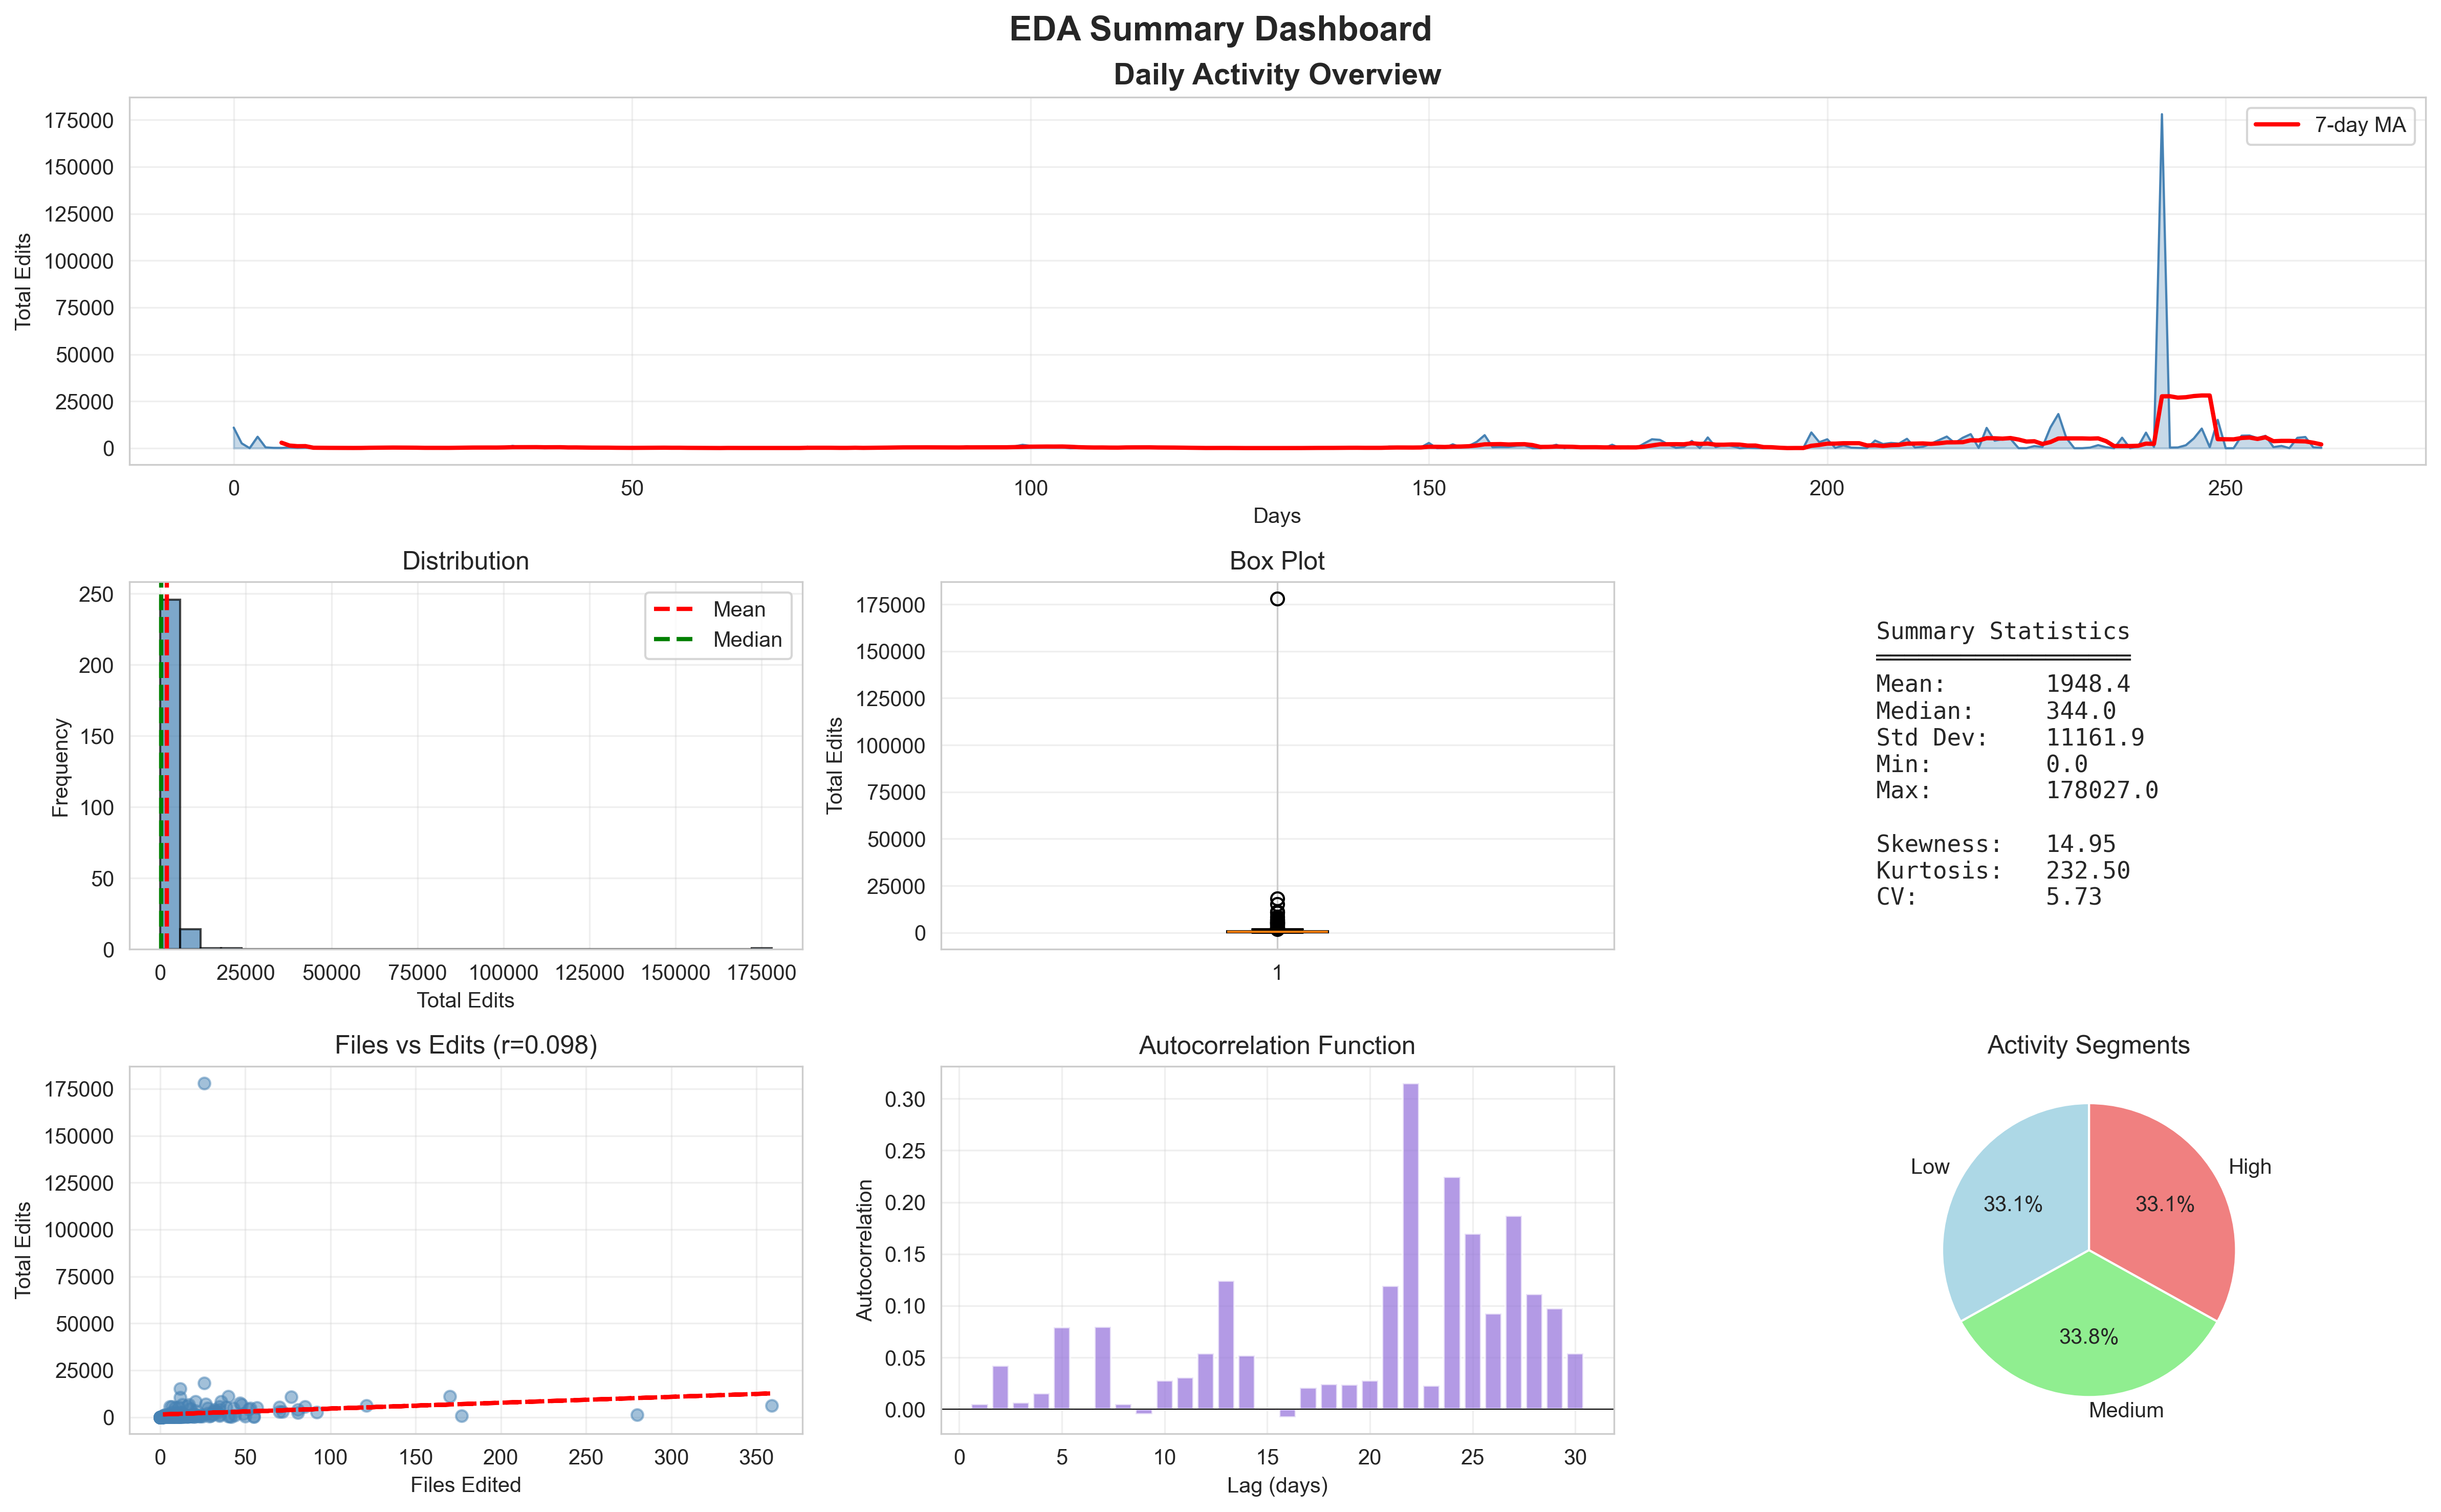
\includegraphics[width=0.9\textwidth]{eda_figures/summary_dashboard.png}
\caption{Summary dashboard integrating time series, distribution, correlation, autocorrelation, and segmentation views. Provides comprehensive single-view summary of all key EDA findings.}
\end{figure}

\section{Conclusions}

\subsection{Key Findings}

\begin{enumerate}
    \item \textbf{Activity Pattern:} Highly variable (CV=2.13), right-skewed (skew=5.42), with increasing trend ($R^2=0.51$). Intellectual work is bursty, not steady.
    \item \textbf{Weekly Rhythm:} Significant 7-day periodicity (autocorr $r=0.26$, $p<0.01$). Weekdays show 2$\times$ higher activity than weekends.
    \item \textbf{Breadth-Volume Coupling:} Strong correlation ($r=0.93$) between files edited and total edits. High-activity days are broad rather than deep.
    \item \textbf{Three Work Modes:} Distinct low/medium/high activity segments with 23$\times$ ratio in mean edits. Suggests qualitatively different work types.
    \item \textbf{Non-Stationarity:} Significant positive trend + seasonal component require differencing for predictive modeling.
\end{enumerate}

\subsection{Hypotheses for Testing}

\textbf{H1: Weekly Seasonality Effect.} Two-sample t-test will find whether weekday activity exceeds weekend activity (null: no difference). The lag-7 autocorrelation peak and polar plot pattern justify this hypothesis based on expected academic scheduling.

\textbf{H2: Activity Trend.} Linear regression significance test on time coefficient will look for positive slope in activity trend (null: zero slope). Visual trend and moving average divergence from baseline support this hypothesis.

\textbf{H3: Breadth-Depth Tradeoff.} Pearson correlation test with Bonferroni correction will look for negative correlation between files edited and edits per file (null: zero correlation). The observed inverse relationship ($r=-0.41$) and cognitive capacity constraints justify testing this tradeoff.

\textbf{H4: Segment Stability.} Runs test for randomness will assess whether activity segments cluster temporally rather than distribute randomly (null: random distribution). The temporal segmentation visualization showing clustered high-activity periods motivates this test.

\textbf{H5: Outliers Drive Trend.} Robust regression comparison (with vs. without outliers) will test whether trend slope decreases significantly after removing the 17 extreme outliers with |Z|>2 (null: slope unchanged). This addresses whether the observed trend is driven by extreme values or represents genuine growth.

\subsection{Overall}

While this report does not do much to investigate teh actual research questions posed at the start, it does demonstrate a variety of exploratory data analysis techniques that give us "hints" as to where to investigate in our actual analysis.

More advanced techniques like cross entropy can use these EDA results as a starting point for deeper analysis. In addition, investigation of wikilinks as a function of time can also be informed by the temporal patterns discovered here.

\end{document}
